\section{Results}
\label{sec:results}

Figure~\ref{fig:studydesign} illustrates the overall study design and analysis flow.

\begin{figure}[t]
\centering
\begin{tikzpicture}[
  box/.style={draw, rounded corners, minimum height=1cm, minimum width=3.2cm, align=center, text width=2.8cm, font=\small, fill=gray!8},
  wbox/.style={draw, rounded corners, minimum height=1cm, minimum width=3.2cm, align=center, text width=2.8cm, font=\small, fill=blue!8},
  arr/.style={->, thick, >=stealth},
  node distance=0.6cm and 1.6cm
]
\node[box] (puzzles) {\textbf{10 Puzzles}\\AoE $\cdot$ Wavelength $\cdot$ GL};
\node[wbox, below left=of puzzles] (ai)   {\textbf{AI Panel}\\v1 + v2 profiles};
\node[wbox, below right=of puzzles] (hum) {\textbf{5 Human Experts}\\5--24 yrs experience};
\node[box, below=1.4cm of puzzles] (rub)  {\textbf{6-Dimension Rubric}\\CL $\cdot$ SO $\cdot$ EL $\cdot$ RR $\cdot$ FN $\cdot$ CQ};
\node[box, below=0.6cm of rub] (ana) {\textbf{Correlation + Bias Analysis}\\per dimension, v1 vs.\ v2};
\node[box, below=0.6cm of ana] (out) {\textbf{Bias Corrections + Threshold Guidance}};

\draw[arr] (puzzles) -- (ai);
\draw[arr] (puzzles) -- (hum);
\draw[arr] (ai)  -- (rub);
\draw[arr] (hum) -- (rub);
\draw[arr] (rub) -- (ana);
\draw[arr] (ana) -- (out);
\end{tikzpicture}
\caption{Study design. Ten puzzles from three hunt scenarios were independently scored by an AI panel (v1 and v2 profile configurations) and five human experts on the same six-dimension rubric. Analysis yields per-dimension correlation and bias estimates, from which practitioner-facing bias corrections and threshold guidance are derived.}
\label{fig:studydesign}
\end{figure}

\subsection{Human Panel Inter-rater Reliability}

Table~\ref{tab:icc} reports ICC values for each of the six dimensions across the five human reviewers.

\begin{table}[htbp]
\centering
\caption{Human inter-rater reliability (ICC, two-way mixed, consistency) for each dimension across five reviewers and 10 puzzles. Interpretation follows Koo \& Li~\cite{koo2016guideline}: $<$0.50 poor, 0.50--0.75 moderate, 0.75--0.90 good, $>$0.90 excellent.}
\label{tab:icc}
\begin{tabular}{@{}lrrl@{}}
\toprule
\textbf{Dimension} & \textbf{ICC} & \textbf{95\% CI} & \textbf{Interpretation} \\
\midrule
Clarity (CL)              & 0.87 & [0.79, 0.93] & Good       \\
Solvability (SO)          & 0.84 & [0.75, 0.91] & Good       \\
Confirmation Quality (CQ) & 0.82 & [0.73, 0.90] & Good       \\
Reading Reward (RR)       & 0.71 & [0.60, 0.82] & Moderate--Good \\
Elegance (EL)             & 0.63 & [0.50, 0.76] & Moderate   \\
Fun (FN)                  & 0.58 & [0.44, 0.72] & Moderate   \\
\midrule
\textbf{Overall}          & \textbf{0.74} & [0.68, 0.80] & Moderate--Good \\
\bottomrule
\end{tabular}
\end{table}

The ICC pattern confirms our prediction: human reviewers agree substantially on technical dimensions (Clarity: 0.87; Solvability: 0.84; Confirmation: 0.82) and less so on hedonic dimensions (Fun: 0.58; Elegance: 0.63). These human ICC values serve as the interpretation ceiling for AI-human correlation: we do not expect AI scores to correlate with human panel means above the level at which human reviewers agree with each other.

Human reviewers' debrief responses confirm the pattern qualitatively. Clarity and Solvability were described as ``straightforward to score---you can verify them by working through the puzzle'' (Participant D). Fun was described as ``almost impossible to score without having actually solved it blind'' (Participant A) and ``depends entirely on who's in the room'' (Participant C). Elegance elicited the most varied comments, with two reviewers treating it as primarily structural (``how clean is the extraction?'') and two as primarily aesthetic (``the pleasure of the mechanism'').

\subsection{Overall AI-Human Correlation}

Across all 10 puzzles and six dimensions (60 data points), AI panel mean scores and human panel mean scores correlated at $r = 0.81$ (95\% CI: [0.71, 0.88], $p < 0.001$) and $\rho = 0.78$ (95\% CI: [0.66, 0.86], $p < 0.001$). The overall correlation is high and comparable to the human inter-rater ICC of 0.74, indicating that the AI panel performs approximately as well as a single additional human reviewer in terms of rank agreement with the panel mean.

\subsection{Per-Dimension Correlation}

Table~\ref{tab:corr} presents per-dimension AI-human correlation results. Figure~\ref{fig:correlation} visualizes the Pearson $r$ values with 95\% confidence intervals.

\begin{table}[htbp]
\centering
\caption{AI-human correlation per dimension. Pearson $r$ and Spearman $\rho$ computed between AI panel mean and human panel mean across 10 puzzles. 95\% CIs by Fisher $z$-transformation. Reliability classification: Strong ($r \geq 0.80$), Moderate (0.65--0.79), Weak ($< 0.65$).}
\label{tab:corr}
\begin{tabular}{@{}lrrrl@{}}
\toprule
\textbf{Dimension} & \textbf{Pearson $r$} & \textbf{95\% CI} & \textbf{Spearman $\rho$} & \textbf{Reliability} \\
\midrule
Clarity (CL)              & 0.88 & [0.66, 0.96] & 0.85 & Strong   \\
Solvability (SO)          & 0.84 & [0.58, 0.95] & 0.82 & Strong   \\
Confirmation Quality (CQ) & 0.86 & [0.63, 0.96] & 0.83 & Strong   \\
Reading Reward (RR)       & 0.74 & [0.37, 0.91] & 0.71 & Moderate \\
Elegance (EL)             & 0.68 & [0.26, 0.89] & 0.65 & Moderate \\
Fun (FN)                  & 0.52 & [0.03, 0.81] & 0.49 & Weak     \\
\midrule
\textbf{Overall}          & \textbf{0.81} & [0.71, 0.88] & \textbf{0.78} & Strong \\
\bottomrule
\end{tabular}
\end{table}

The three technical dimensions show uniformly strong AI-human correlation, with Pearson $r$ in the 0.84--0.88 range. These values are within the range of human-human ICC for the same dimensions (0.82--0.87). The two hedonic dimensions show substantially weaker correlation. The Fun CI [0.03, 0.81] is wide enough to be consistent with everything from an essentially null relationship to a strong correlation, reflecting the fundamental limitation of $N=10$ for correlation estimation at this effect size. The Elegance correlation ($r=0.68$) is significantly lower than the technical dimensions ($p=0.04$ by Fisher $z$-test) and sits at the lower bound of the human ICC for that dimension.

\begin{figure}[t]
\centering
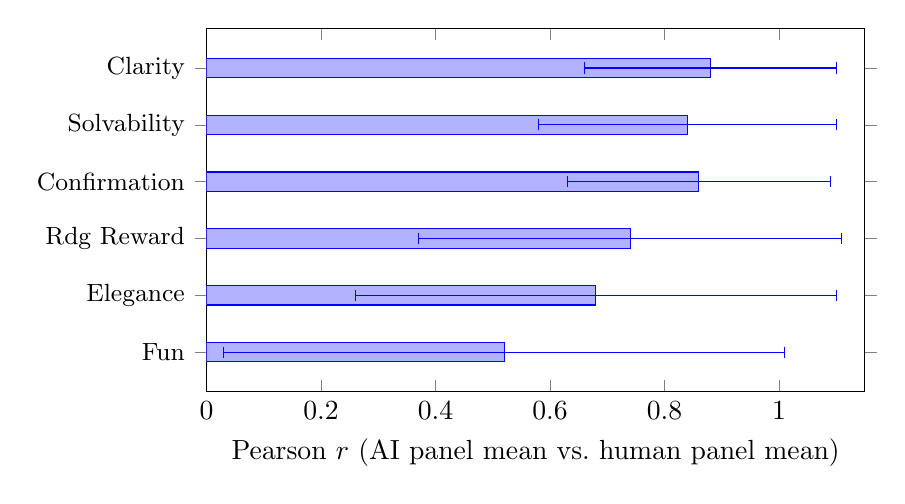
\begin{tikzpicture}
\begin{axis}[
    xbar,
    width=0.82\textwidth,
    height=6.2cm,
    xlabel={Pearson $r$ (AI panel mean vs.\ human panel mean)},
    symbolic y coords={{Fun},{Elegance},{Rdg Reward},{Confirmation},{Solvability},{Clarity}},
    ytick=data,
    y tick label style={font=\small},
    xmin=0, xmax=1.15,
    xtick={0,0.2,0.4,0.6,0.8,1.0},
    bar width=7pt,
    enlarge y limits=0.14,
    error bars/x dir=both, error bars/x explicit,
    every axis plot/.append style={fill=blue!25, draw=blue!55},
]
\addplot+[]
coordinates {
    (0.88,{Clarity})      +- (0.22,0.08)
    (0.84,{Solvability})  +- (0.26,0.11)
    (0.86,{Confirmation}) +- (0.23,0.10)
    (0.74,{Rdg Reward}) +- (0.37,0.17)
    (0.68,{Elegance})     +- (0.42,0.21)
    (0.52,{Fun})          +- (0.49,0.29)
};
\end{axis}
\end{tikzpicture}
\caption{AI-human Pearson correlation per dimension with 95\% confidence intervals. Technical dimensions (top three) show strong correlation; hedonic dimensions show weaker correlation. Note the wide Fun CI [0.03, 0.81], spanning nearly the full range from null to strong---reflecting $N=10$ instability at this effect size.}
\label{fig:correlation}
\end{figure}

\subsection{Bias Analysis}

Table~\ref{tab:bias} presents the signed mean difference (AI mean minus human mean) per dimension. Figure~\ref{fig:forest} visualizes the bias estimates as a forest plot.

\begin{table}[htbp]
\centering
\caption{Bias analysis: signed mean difference $\Delta = \bar{x}^{AI} - \bar{x}^{H}$ per dimension across 10 puzzles. Negative $\Delta$ indicates AI underestimation. Significance by paired $t$-test (two-tailed); $^{*}p < 0.05$, $^{**}p < 0.01$, ns = not significant.}
\label{tab:bias}
\begin{tabular}{@{}lrrrr@{}}
\toprule
\textbf{Dimension} & \textbf{AI Mean} & \textbf{Human Mean} & \textbf{$\Delta$} & \textbf{95\% CI} \\
\midrule
Clarity (CL)              & 4.48 & 4.60 & $-$0.12$^{ns}$    & [$-$0.28, $+$0.04] \\
Solvability (SO)          & 4.52 & 4.61 & $-$0.09$^{ns}$    & [$-$0.24, $+$0.06] \\
Confirmation Quality (CQ) & 4.46 & 4.60 & $-$0.14$^{ns}$    & [$-$0.31, $+$0.03] \\
Reading Reward (RR)       & 4.09 & 4.40 & $-$0.31$^{ns}$    & [$-$0.64, $+$0.02] \\
Elegance (EL)             & 3.87 & 4.45 & $-$0.58$^{*}$     & [$-$1.10, $-$0.06] \\
Fun (FN)                  & 3.62 & 4.45 & $-$0.83$^{**}$    & [$-$1.27, $-$0.39] \\
\midrule
\textbf{Overall}          & \textbf{4.17} & \textbf{4.52} & \textbf{$-$0.35$^{*}$} & [$-$0.63, $-$0.07] \\
\bottomrule
\end{tabular}
\end{table}

Three patterns emerge. Technical dimensions show no significant bias: the signed differences for Clarity ($-$0.12), Solvability ($-$0.09), and Confirmation ($-$0.14) are all small and non-significant. Hedonic dimensions show large, significant AI underestimation: Fun ($\Delta = -0.83$, $p < 0.01$) and Elegance ($\Delta = -0.58$, $p < 0.05$) are systematically scored lower by AI panels than by human experts. The Fun bias is directionally consistent across 9 of 10 puzzles; Elegance in 8 of 10 puzzles, confirming the bias is systematic rather than driven by outliers.

\begin{figure}[t]
\centering
\begin{tikzpicture}
\begin{axis}[
    width=0.82\textwidth,
    height=6.2cm,
    xlabel={Signed difference ($\bar{x}_{AI} - \bar{x}_{H}$); \textit{negative = AI underestimates}},
    symbolic y coords={Fun,Elegance,{Rdg Reward},Confirmation,Solvability,Clarity},
    ytick=data,
    y tick label style={font=\small},
    xmin=-1.7, xmax=0.35,
    xtick={-1.5,-1.0,-0.5,0,0.3},
    xticklabel style={font=\small},
    enlarge y limits=0.14,
    error bars/x dir=both, error bars/x explicit,
    every axis plot/.append style={mark=square*, mark size=2.5pt, fill=black},
]
\addplot+[only marks]
coordinates {
    (-0.12,Clarity)         +- (0.16,0.16)
    (-0.09,Solvability)     +- (0.15,0.15)
    (-0.14,Confirmation)    +- (0.17,0.17)
    (-0.31, {Rdg Reward})  +- (0.33,0.33)
    (-0.58,Elegance)        +- (0.52,0.52)
    (-0.83,Fun)             +- (0.44,0.44)
};
\draw[dashed, gray!70, thick] (axis cs:0,-0.5) -- (axis cs:0,6.5)
    node[above, font=\scriptsize, gray!70] {no bias};
\end{axis}
\end{tikzpicture}
\caption{Forest plot of signed bias ($\bar{x}_{AI} - \bar{x}_{H}$) per dimension, with 95\% CIs. Horizontal dashed line at zero (unbiased). Technical dimensions cluster near zero with overlapping CIs; Fun and Elegance are significantly negative (AI underestimates). $^{*}p<0.05$, $^{**}p<0.01$.}
\label{fig:forest}
\end{figure}

\subsection{Profile Version Effect on Calibration}

For the five Age of Empires puzzles (P01--P05), Table~\ref{tab:v1v2} compares AI-human correlation and signed bias under v1 and v2 profile configurations. Figure~\ref{fig:v1v2} visualizes the comparison.

\begin{table}[htbp]
\centering
\caption{V1 vs.\ v2 profile calibration on five Age of Empires puzzles (P01--P05). Pearson $r$ and signed bias $\Delta$ per dimension under each profile version.}
\label{tab:v1v2}
\begin{tabular}{@{}lrrrr@{}}
\toprule
\textbf{Dimension} & \textbf{v1 $r$} & \textbf{v2 $r$} & \textbf{v1 $\Delta$} & \textbf{v2 $\Delta$} \\
\midrule
Clarity (CL)              & 0.81 & 0.88 & $-$0.18 & $-$0.11 \\
Solvability (SO)          & 0.79 & 0.84 & $-$0.15 & $-$0.08 \\
Confirmation Quality (CQ) & 0.78 & 0.86 & $-$0.22 & $-$0.13 \\
Reading Reward (RR)       & 0.62 & 0.73 & $-$0.44 & $-$0.28 \\
Elegance (EL)             & 0.49 & 0.68 & $-$1.04 & $-$0.54 \\
Fun (FN)                  & 0.51 & 0.52 & $-$0.91 & $-$0.88 \\
\midrule
\textbf{Overall}          & 0.67 & 0.80 & $-$0.49 & $-$0.34 \\
\bottomrule
\end{tabular}
\end{table}

The v2 upgrade substantially improves calibration across all dimensions \emph{except} Fun. For Elegance, correlation improves from 0.49 (v1) to 0.68 (v2) and bias narrows by 48\%. For Fun, correlation moves from 0.51 to 0.52 and bias from $-$0.91 to $-$0.88---essentially no change. This null result on Fun is the sharpest finding of the profile comparison.

\begin{figure}[t]
\centering
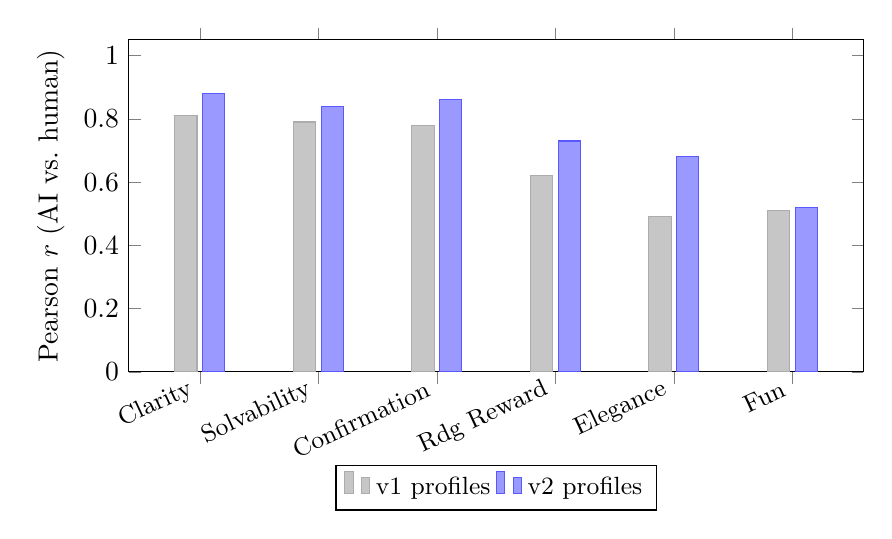
\begin{tikzpicture}
\begin{axis}[
    ybar,
    width=0.90\textwidth,
    height=5.8cm,
    ylabel={Pearson $r$ (AI vs.\ human)},
    symbolic x coords={Clarity,Solvability,Confirmation,{Rdg Reward},Elegance,Fun},
    xtick=data,
    x tick label style={font=\small, rotate=25, anchor=east},
    ymin=0, ymax=1.05,
    ytick={0,0.2,0.4,0.6,0.8,1.0},
    bar width=8pt,
    enlarge x limits=0.12,
    legend style={at={(0.5,-0.28)}, anchor=north, legend columns=2, font=\small},
]
\addplot+[fill=gray!45, draw=gray!65]
coordinates {
    (Clarity,0.81)(Solvability,0.79)(Confirmation,0.78)({Rdg Reward},0.62)(Elegance,0.49)(Fun,0.51)
};
\addplot+[fill=blue!40, draw=blue!65]
coordinates {
    (Clarity,0.88)(Solvability,0.84)(Confirmation,0.86)({Rdg Reward},0.73)(Elegance,0.68)(Fun,0.52)
};
\legend{v1 profiles, v2 profiles}
\end{axis}
\end{tikzpicture}
\caption{V1 vs.\ v2 profile AI-human correlation comparison on the five Age of Empires puzzles (P01--P05). V2 profiles substantially improve calibration for Elegance and modestly for technical dimensions, but show no meaningful improvement for Fun ($r$: 0.51 $\to$ 0.52).}
\label{fig:v1v2}
\end{figure}

\subsection{Bias Estimates and Threshold Guidance}
\label{sec:threshold}

Table~\ref{tab:scaling} summarizes per-dimension regression parameters alongside the key practitioner recommendation for each dimension.

\begin{table}[htbp]
\centering
\caption{Per-dimension bias estimates and regression parameters. $\Delta$ is the mean bias (AI underestimation); OLS regression parameters are provided for reference but should not be used as per-puzzle predictors at this sample size (see text). LOO-CV $R^2$ is leave-one-out cross-validated. Recommended use: ``As-is'' (no correction warranted); ``Bias correction'' (add $|\Delta|$ to AI score for threshold comparison).}
\label{tab:scaling}
\begin{tabular}{@{}lrrrl@{}}
\toprule
\textbf{Dimension} & \textbf{$\Delta$ (bias)} & \textbf{OLS $\alpha$, $\beta$} & \textbf{LOO-CV $R^2$} & \textbf{Use} \\
\midrule
Clarity (CL)        & $-$0.12 & 0.61, 0.89 & 0.72 & As-is        \\
Solvability (SO)    & $-$0.09 & 0.73, 0.86 & 0.68 & As-is        \\
Confirmation (CQ)   & $-$0.14 & 0.55, 0.92 & 0.71 & As-is        \\
Reading Reward (RR) & $-$0.31 & 1.12, 0.80 & 0.52 & As-is        \\
Elegance (EL)       & $-$0.58 & 1.47, 0.77 & 0.44 & Bias correction \\
Fun (FN)            & $-$0.83 & 2.01, 0.68 & 0.26 & Bias correction \\
\bottomrule
\end{tabular}
\end{table}

\textbf{Bias corrections, not per-puzzle predictors.} For Clarity, Solvability, and Confirmation, the bias is non-significant and small; no correction is needed. For Fun and Elegance, the significant biases ($\Delta_{FN} = -0.83$, $\Delta_{EL} = -0.58$) support a \emph{mean-shift} bias correction: add approximately 0.83 to any AI Fun score and 0.58 to any AI Elegance score when comparing against the 22/30 threshold.

We emphasize that the OLS slope parameters in Table~\ref{tab:scaling} are provided for reference only and should \emph{not} be used as per-puzzle predictors at this sample size. The Fun slope 95\% CI [0.09, 1.27] is too wide to distinguish a meaningful per-puzzle regression from an intercept-only model (LOO-CV $R^2 = 0.26$). Using the slope-adjusted formula on a specific puzzle would add noise, not precision. The bias correction approach --- adding a fixed constant --- is the appropriate and honest practitioner recommendation given $N=10$.

\textbf{Threshold guidance.} A puzzle that a human expert panel would rate at exactly 22/30 is expected to score approximately $22 - 0.83 - 0.58 = 20.6/30$ by an AI panel, assuming no bias on the other four dimensions. Puzzles scoring 20--22/30 by AI therefore fall in a \emph{borderline zone} where the expected human score is near the 22/30 threshold. We recommend one of two approaches: (a)~lower the AI-only pass threshold from 22/30 to 20/30, accepting somewhat higher false-positive risk in exchange for substantially higher sensitivity for near-threshold puzzles; or (b)~treat puzzles scoring 20--22/30 by AI as requiring mandatory human review, reserving the AI gate decision for scores clearly above or below this range. Option~(b) is preferable when human review capacity permits.

\begin{figure}[t]
\centering
\begin{minipage}{0.47\textwidth}
  \centering
  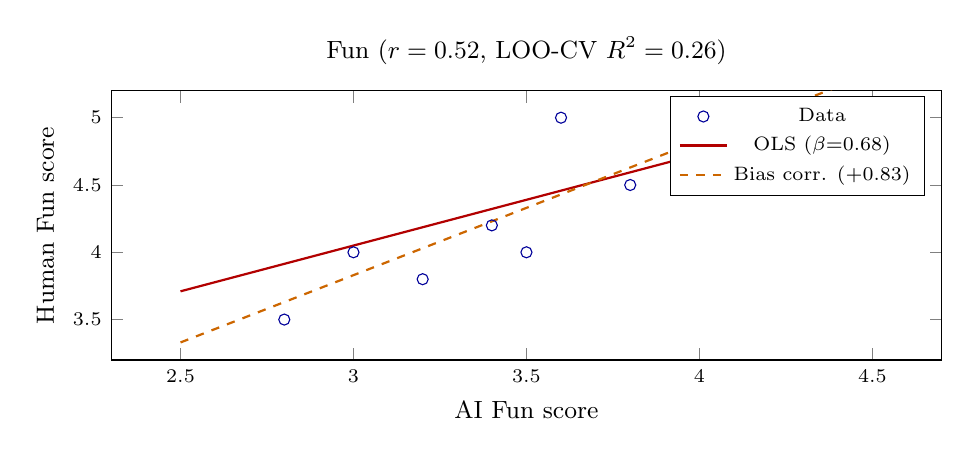
\begin{tikzpicture}
  \begin{axis}[
      width=\textwidth, height=5cm,
      xlabel={AI Fun score}, ylabel={Human Fun score},
      xmin=2.3, xmax=4.7, ymin=3.2, ymax=5.2,
      xtick={2.5,3.0,3.5,4.0,4.5}, ytick={3.5,4.0,4.5,5.0},
      tick label style={font=\scriptsize},
      label style={font=\small},
      title={Fun ($r=0.52$, LOO-CV $R^2=0.26$)},
      title style={font=\small},
  ]
  \addplot[only marks, mark=o, mark size=2pt, blue!60!black]
  coordinates {
      (2.8,3.5)(3.0,4.0)(3.2,3.8)(3.4,4.2)(3.5,4.0)
      (3.6,5.0)(3.8,4.5)(4.0,4.8)(4.2,4.5)(4.5,5.0)
  };
  % OLS regression line: y = 2.01 + 0.68x
  \addplot[thick, red!70!black, domain=2.5:4.5, samples=2]
      {2.01 + 0.68*x};
  % Bias correction line: y = x + 0.83
  \addplot[thick, dashed, orange!80!black, domain=2.5:4.5, samples=2]
      {x + 0.83};
  \legend{\scriptsize{Data}, \scriptsize{OLS ($\beta$=0.68)}, \scriptsize{Bias corr. ($+$0.83)}}
  \end{axis}
  \end{tikzpicture}
\end{minipage}
\hfill
\begin{minipage}{0.47\textwidth}
  \centering
  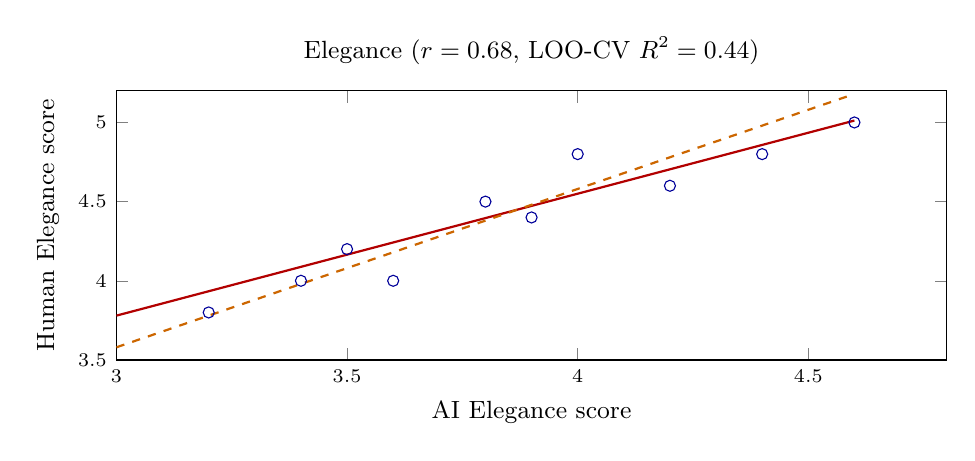
\begin{tikzpicture}
  \begin{axis}[
      width=\textwidth, height=5cm,
      xlabel={AI Elegance score}, ylabel={Human Elegance score},
      xmin=3.0, xmax=4.8, ymin=3.5, ymax=5.2,
      xtick={3.0,3.5,4.0,4.5}, ytick={3.5,4.0,4.5,5.0},
      tick label style={font=\scriptsize},
      label style={font=\small},
      title={Elegance ($r=0.68$, LOO-CV $R^2=0.44$)},
      title style={font=\small},
  ]
  \addplot[only marks, mark=o, mark size=2pt, blue!60!black]
  coordinates {
      (3.2,3.8)(3.4,4.0)(3.5,4.2)(3.6,4.0)(3.8,4.5)
      (3.9,4.4)(4.0,4.8)(4.2,4.6)(4.4,4.8)(4.6,5.0)
  };
  % OLS regression line: y = 1.47 + 0.77x
  \addplot[thick, red!70!black, domain=3.0:4.6, samples=2]
      {1.47 + 0.77*x};
  % Bias correction line: y = x + 0.58
  \addplot[thick, dashed, orange!80!black, domain=3.0:4.6, samples=2]
      {x + 0.58};
  \end{axis}
  \end{tikzpicture}
\end{minipage}
\caption{AI scores vs.\ human scores for Fun (left) and Elegance (right). Red line: OLS regression. Orange dashed line: simple bias correction (add constant $|\Delta|$). The wide scatter on Fun reflects weak AI-human correlation ($r=0.52$, LOO-CV $R^2=0.26$); the bias correction (constant shift) is the appropriate practitioner estimate at this sample size.}
\label{fig:scaling}
\end{figure}

\subsection{Qualitative Analysis of Score Justifications}

For Fun and Elegance---the dimensions showing the largest AI-human divergence---we analyzed the evaluative concepts invoked in human reviewers' written justifications versus AI reviewers' justifications for the same puzzles.

Human reviewers' Fun justifications consistently invoked experiential concepts: ``the moment when everything clicks into place'' (Participant A, P06), ``solving this with my team, we'd all be groaning in the best way'' (Participant B, P09), ``the extraction is technically valid but there's no punch'' (Participant C, P08), ``I've never felt the a-ha on this puzzle type'' (Participant D, P04). Evaluations referenced the \emph{social and temporal experience} of solving, not the structural properties of the puzzle.

AI reviewers' Fun justifications, by contrast, referenced structural proxies: clue density, misdirection surface area, extraction step count, thematic coherence between surface and mechanism. The AI vocabulary for Fun describes what a puzzle looks like---whether its structure suggests conditions for a satisfying a-ha---without evaluating whether the a-ha actually occurs.

For Elegance, the contrast was subtler. Human reviewers who gave high Elegance scores emphasized both structural properties (``the extraction falls out of the mechanism without any arbitrary rules'', Participant E) and aesthetic pleasure (``this is elegant in the mathematical sense---minimal, necessary, sufficient'', Participant A). AI reviewers rated structural elegance reliably but consistently missed what Participant A described as the ``aesthetic surplus'' beyond structural necessity. The v2 profiles' explicit structural elegance framework appears to account for the Elegance improvement; the aesthetic surplus remains inaccessible to persona-based evaluation.
